\section{Method}
\label{method}
Past research has established the importance of rapid serial visual presentation (RSVP), for the understanding cognition and memory processing, spatio-temporal localization of neural synchronizations following stimuli, and for most brain-computer interfaces (BCI). Reading is a ubiquitous daily activity, which links to these three aforementioned fields.  As online (mostly written) content production has exploded \cite{something about reading more with the Internet}, finding ways for people to read more and faster shall therefore become a sound economic goal. RSVP systems like {\it Spritz} \cite{} or {\it Spreeder} \cite{} go in this direction, but these implementations currently lack an efficient, ubiquitous control of display rate, as noted early by Potter (Applied Questions About RSVP, p114-115 \cite{potter1984rapid}). Since neural activity associated with cognitive effort can be captured by EEG, a BCI for controlling the display rate is a good candidate to overcome this problem. Nonetheless, the BCI interface shall be as cheap as possible to ensure widespread adoption.

\subsection{Hypotheses}
\label{hypo}
Here, we design our {\it brain speed reader} under the following set of constraints: (i) ubiquitous control through BCI, by taking into account (ii) cognitive aspects of reading, and (iii) ensuring the lowest possible implementation and operational costs. In other words, given that the noise-to-signal ratio is an inverse function of EEG sophistication, equipment price and operation costs, we shall design an apparatus, which delivers the minimal meaningful signal to ensure a satisfactory control of the word display rate.

For that, we set hypotheses of relations between cognitive activity associated with reading, and the control of word display rate. Increased cognitive activity, involving (conceptual) short-term, working, long-term memory, are reflected by increased neuronal synchronization, in short \cite{} and large frequency ranges \cite{}. \textcolor{red}{be more specific here}. We build on these results to propose two working hypotheses to link the attention measured as the increase of brain synchronization, and of word display in the rapid serial visual presentation (RSVP) setting. The conservative hypothesis is the higher the attention, the slower the word-pace, so that the brain is given enough time to process information (causality between the nature of the text read, and brain processing).


{\bf Hypothesis 1a: }  the higher the cognitive activity, the slower the word-pace, 

On the contrary, we aim also to test whether the high attention state benefits fast reading (reverse causality) \textcolor{red}{\bf [any reference on this ?]}. In that case, the prior is the level of brain attention, which in turn enables faster integration of knowledge read through RSVP.

{\bf Hypothesis 1b:} the higher the cognitive activity, the faster the word-pace

Even though, we (assume) we cannot observe reliably the lag observed during knowledge integration by the brain (usually 200-400ms), we shall consider that it has an influence on the design of {\it brain speed reader}, based on RSVP at a usual pace of 100-150 ms/word. So the speed of word presentation shall be adapted smoothly to account for this lag.

{\bf Hypothesis 2:} because the typical lag for knowledge integration from reading may be twice as large as the RSVP typical word exposure time, we shall determine an optimal speed of rate change (derivative of rate, i.e. second derivative of instant presentation time).

{\bf In this study, our overall goal is to find the most comfortable configuration of (i) rate and (ii) adaptability, over a large population, and explain the potential variance at the individual level from control variables.}

In the rest of the Method section, we shall describe successively, (i) the entropy-based signal processing method we have used to measure brain (neural) synchronization, (ii) the apparatus, (iii) the experimental protocol and data collected.

\subsection{EEG Signal Processing \& Entropy}
In general, there are two approaches to analyze EEG signal:  (i) a spatio-temporal method, mainly guided by the detection of event-related potentials (ERPs), and (ii) spectral analysis. The former appears too sensitive to be reliably used in a consistent way with a single-channel dry consumer-grade EEG, such as the Neurosky Mindwave \cite{}. To account for dynamics of brain synchronization in the spectral domain, every 0.25 second we analyze the frequency domain $0-128Hz$ (the hardware sampling rate is 512 Hz), by computing the power spectrum density associated with the Fourier transform of the signal over each period. Figure \ref{fig:pspectrum} shows typical power spectrum densities, associated with simple tasks, such as {\it resting state} (i.e. closed eyes, no mental focus) \cite{}, {\it passively watch a screen (with a video?)}, and read a text in English on the same screen, in silence and loud. We see that the structure of the power spectrum density varies significantly across tasks. This result is consistent also across subjects \textcolor{red}{[\bf bring evidence here.]}.

 \begin{figure}[!t]
\centering
%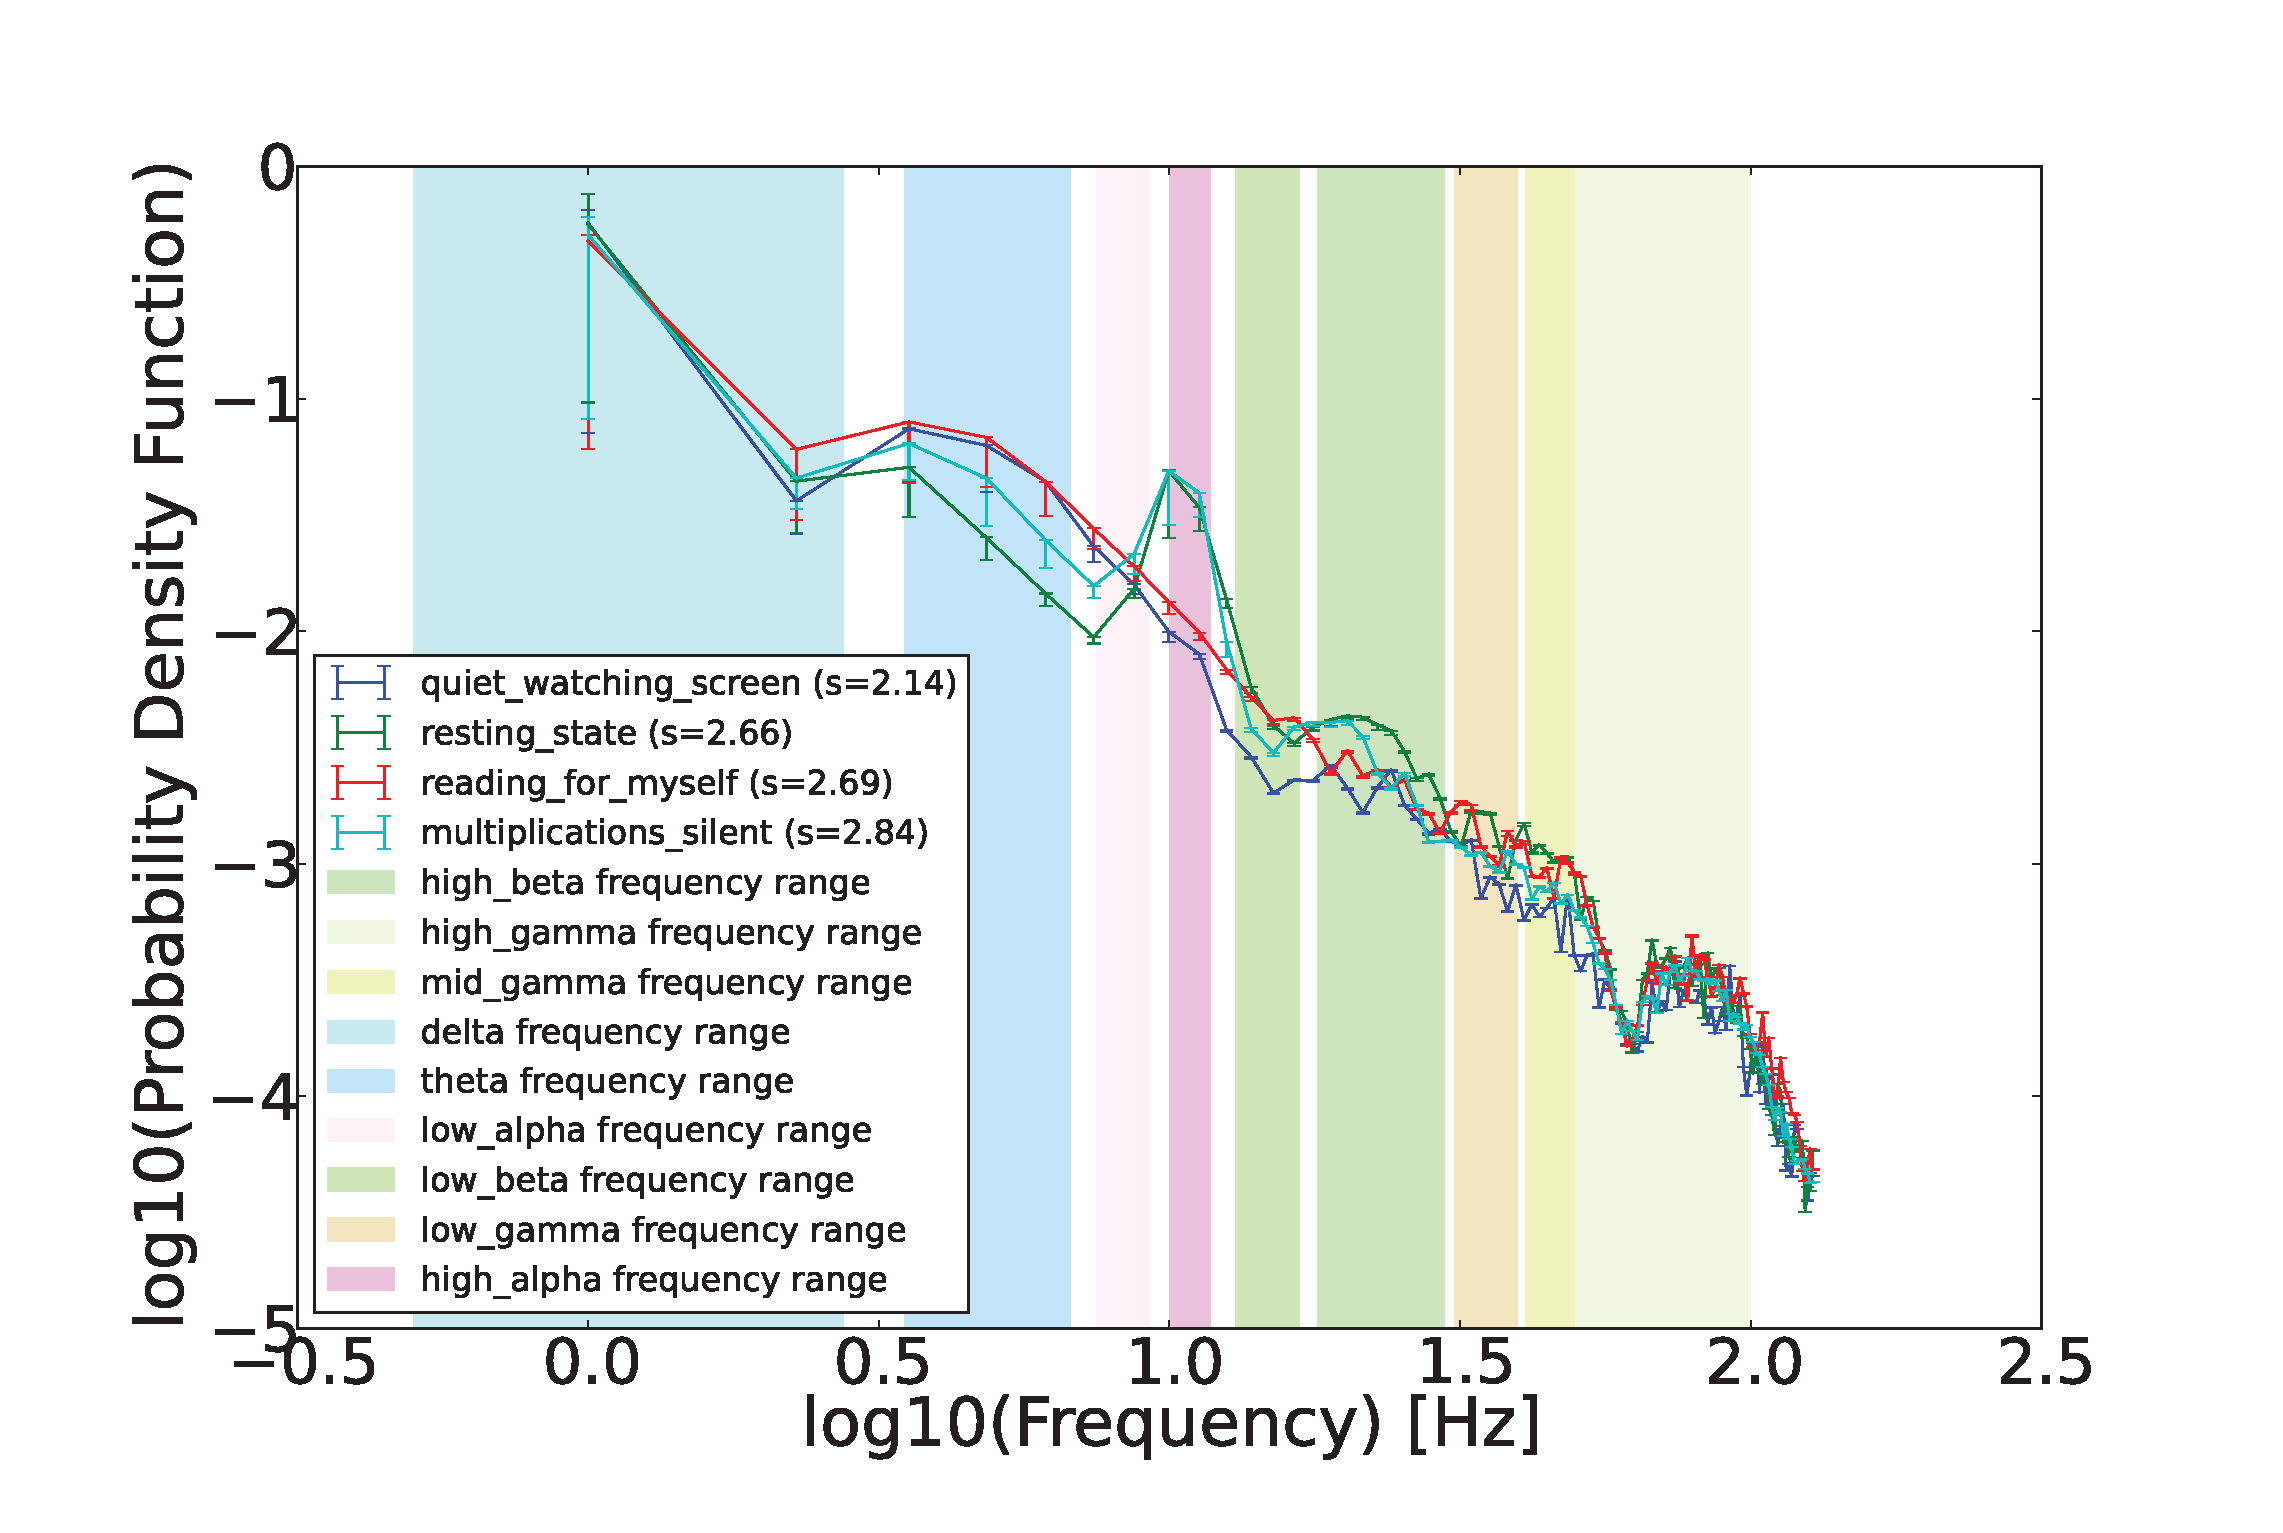
\includegraphics[width=1.1\columnwidth]{../figures/compareArtifacts.eps}
\caption{Show the difference between resting state, being passive in front of a screen, and actively reading a text, in double logarithmic scale.}
\label{fig:pspectrum}
\end{figure}

Figure \ref{fig:pspectrum} shows the heavy-tailed distribution of the power spectrum density, approximately a straight line in double logarithmic scale, which corresponds to current understanding of the pink noise nature of brain synchronization, $pdf(f) \sim 1/f^{\mu+1}$, with $f$ the frequency and $\mu \approx 1$ \cite{pink noise brain}.

From previous research, we know that the density of the power spectrum increases in case of increased cognitive activity \cite{}, in particular in the case of reading a text, which is of interest here \cite{}. 

Entropy is one simple and non-parametric way to account for the variation of power spectrum density function$pdf(f)$. The simplest and most common entropy metric is the one of Boltzmann for any logarithmic base, or more specifically the entropy of Shannon in base 2, given by,

%\begin{equation}
%\label{eq:tsallis}
%S_q(X) = \frac{1}{q-1} \left[ 1 - \sum_{i=1}^n (p_i)^q \right].
%\end{equation}

\begin{equation}
\label{eq:shannon}
S = - \sum_{i=1}^n p_i\cdot log_{2}(p_i).
\end{equation}

Entropy is a very convenient metric for our purpose, because it represents nothing else than the discrete integral of the logarithmic frequency densities. In other words, it provides a single scalar value, which accounts for all the power spectrum density function $pdf(f)$.\footnote{There are several reasons for not choosing any of the built-in {\it meditation} and {\it attention} metrics provided by Neurosky: (i) these metrics are proprietary, and it is therefore impossible to know what purpose they exactly serve (i.e., what are definitions of meditation and attention according to Neurosky?); (ii) we nevertheless suspect that they take an average of $\alpha$ and $\beta$ frequency ranges as an input, which is more restrictive than our approach, especially given that the ranges of $\alpha$ and $\beta$ frequency may vary from one subject to another when reading \cite{}.} 

Entropy $S$ shall only be seen as a convenient coarse-grained and compressed measure of neural synchronization in the brain over a short period. As we aim to measure variations of synchronization states over time, a relative value of $S$ is accurate. For that, entropy normalized over a short period of time is sufficient to capture short-term variations of neural coherence as a result of cognitive tasks, involving solicitation of short-term memory, and quick recalls of conceptual elements from long-term memory. We therefore define 

\begin{equation}
\label{eq:Snormalized}
S_{norm}(t) = \frac{S(t) - \langle S \rangle}{\sigma_{S}}, 
\end{equation}

with $\langle S \rangle$ and $\sigma_{S}$ the average and standard deviation of the entropy $S$ calculated over the last 20 points (i.e., the last 5 seconds). %By definition, $S_{norm}$ is always centered around $0$.

Like any other measure taking EEG as an input, entropy is subjected to artifacts, in particular eye-blinks. We shall later expose how to reduce, or on the contrary harness, the influence of non-neural artifacts recorded by the EEG. Nevertheless, EEG entropy offers therefore a non-parametric way to compress information contained in the power spectrum density into a single scalar instantaneous value. Normalized entropy $S_{norm}$ ensures that only local variations are captured. 

%We wanted a lightweight mobile apparatus, which does not require complicated machine learning or any communication with a cloud service, or would not drain a battery. We purposely decided for a cheap update method {\bf [continue this point in discussion because it helps introduce future work]}

\section{Apparatus}
The brain speed-reader is an apparatus, which displays words on a screen at variable $r(t)$, which in turn is read by the user. The reading task triggers a change of brain activity, which can be recorded and analyzed through electroencephalograms (EEG). As our apparatus is conceived for use in a naturalistic environment, we have used, {\it Neurosky Mindwave}, the cheapest consumer-grade EEG headset available for less than \$100 on the market. As shown on Figure \ref{fig:apparatus} and explained step-by-step below, the EEG signal is processed online, in order to adapt the rate of words displayed as function of cognitive activity: if the rate $r$ is too large (resp. too low) at time $t$, then reading triggers more  (resp. less) cognitive activity, which in turn allows reducing (resp. increasing) $r$ at $t+1$. In this section, we explain step-by-step the design of the apparatus in details.

\begin{figure}[!t]
\centering
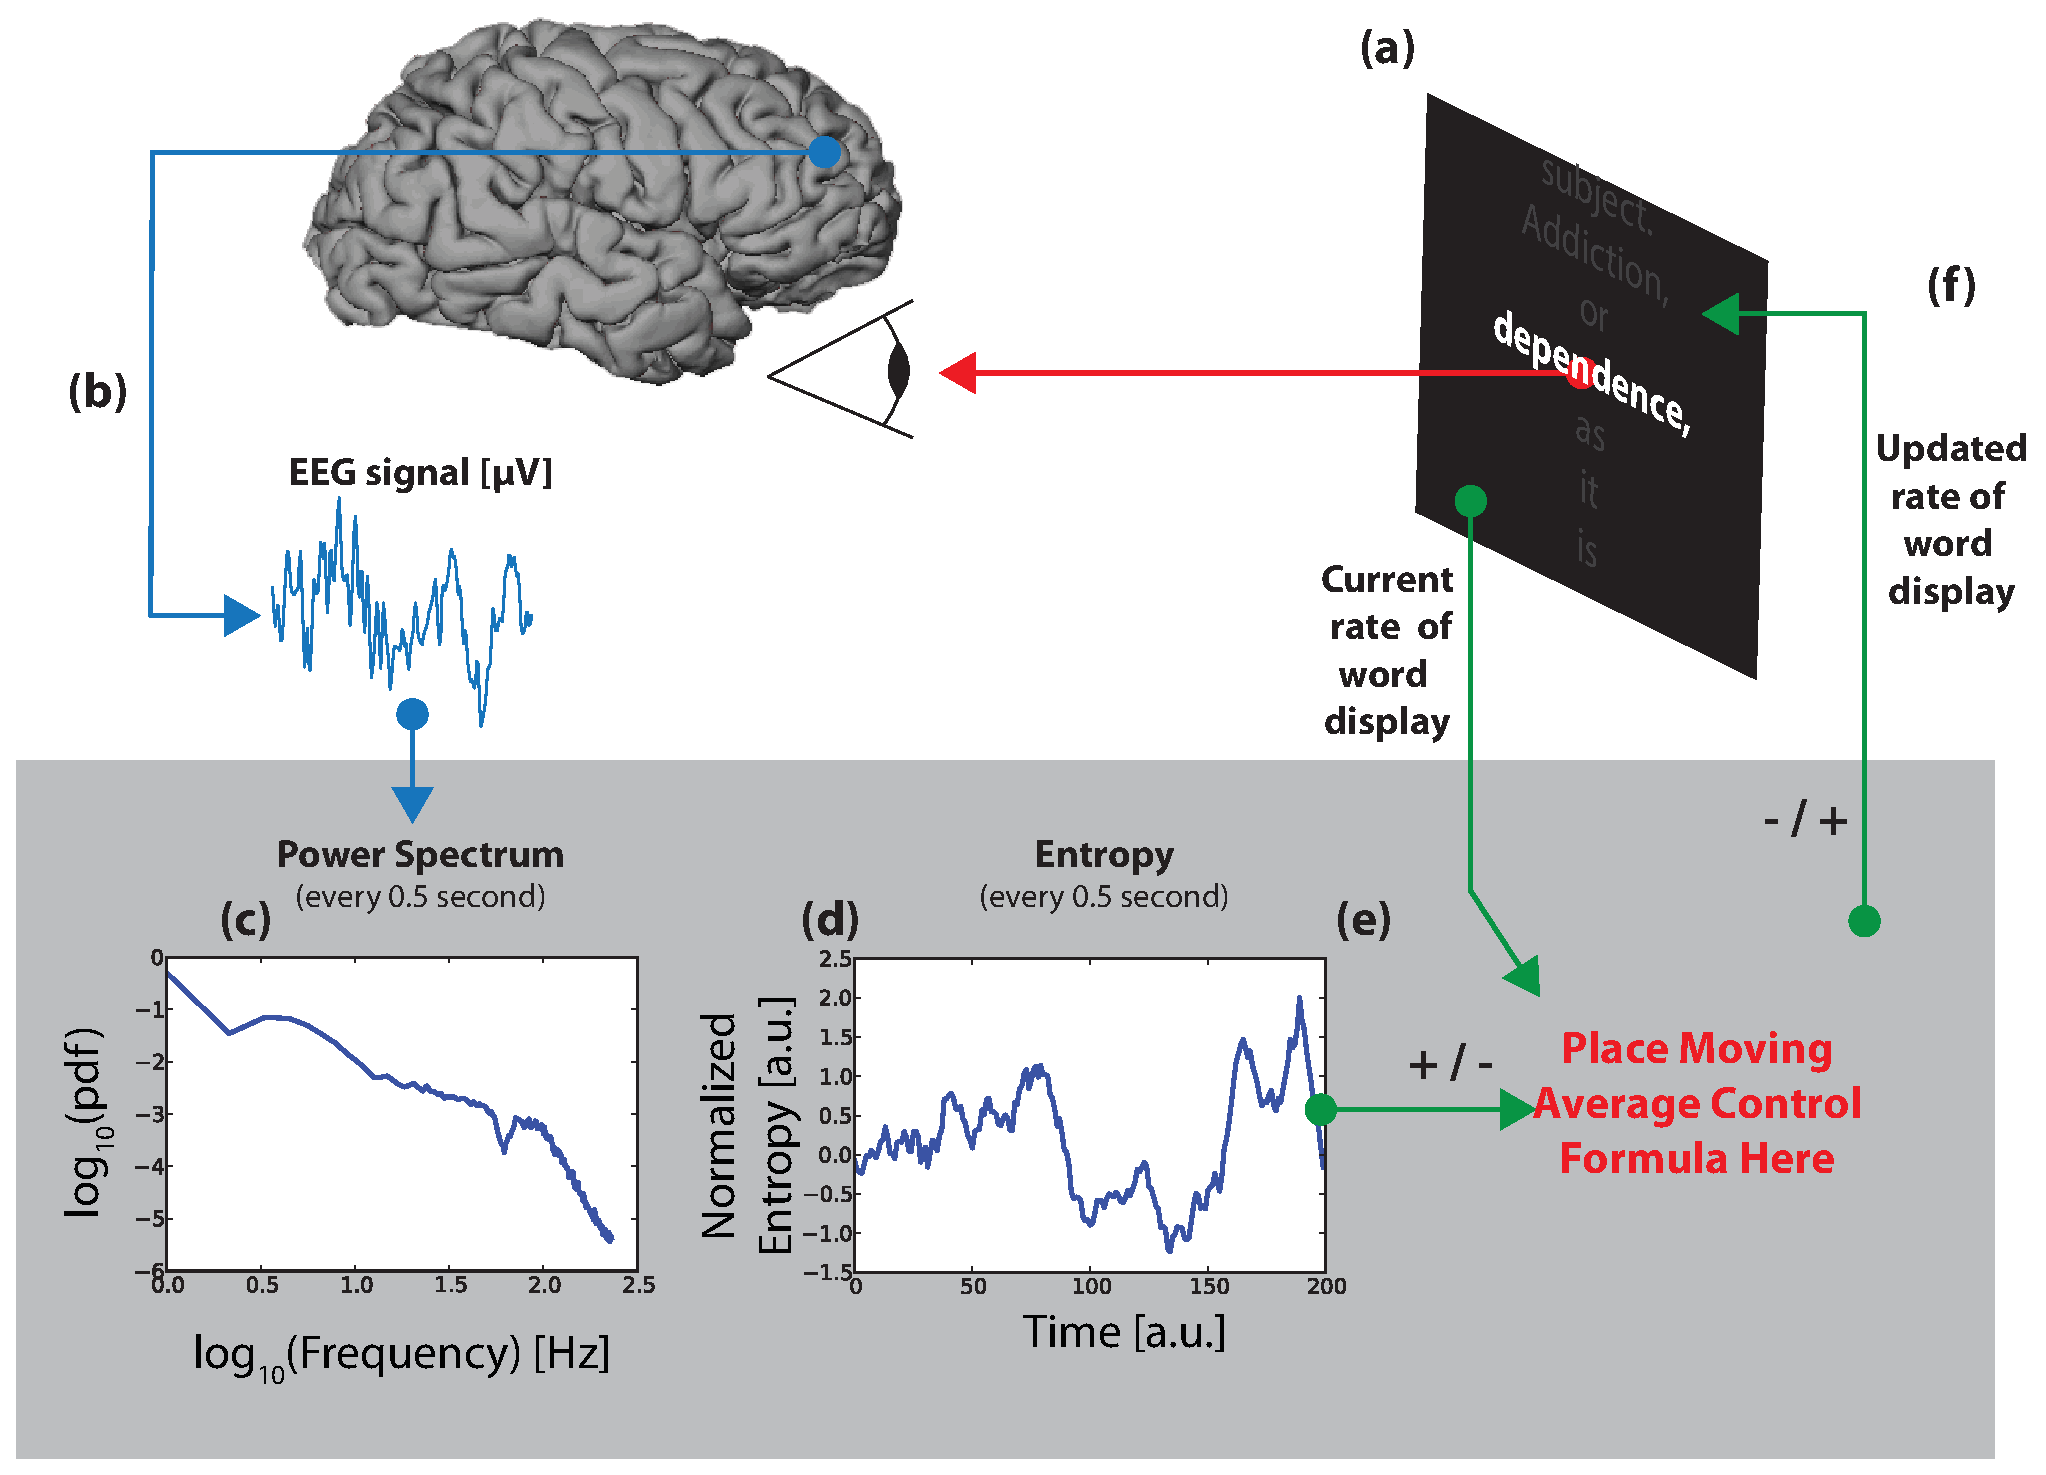
\includegraphics[width=0.9\columnwidth]{../figures/apparatus.eps}
\caption{Brain speed-reader apparatus: {\bf (a)} Words are displayed and read one after the other at a given rate. {\bf (b)} the EEG signal is recorded through a consumer grade device (here the {\it Neurosky Mindwave}). {\bf (c)} The EEG signal is turned every 0.5 seconds into a power spectrum through a Fourier transform, {\bf (d)} the characteristics of the power spectrum are compressed into a single value characteristic entropy $s$ value. {\bf (e)} A new rate of word display is updated by taking into its current value and $s$. {\bf (f)} The rate of word display is updated accordingly.}
\label{fig:apparatus}
\end{figure}

\subsection{Rate of Word Display}
The principle of {\it Rapid Serial Visual Presentation} (RVSP) applied to text, is precisely to display the words of a text at a controlled rate. However, in most RVSP implementations for text, the rate of word display pre-determined and remains constant. In our implementation, the user first calibrates the brain speed-reader by tuning a comfortable baseline word display rate $r_{baseline} = r(t = 0)$. The operation takes only a few seconds. This is a usual way to proceed when using usual text RVSP applications.

\subsection{Brain Activity as Captured by EEG signal}
Unlike traditional text RVSP, we wish to let the user adapt the rate of word display in real-time, through brain activity as captured by EEG signal, to control for a text becoming suddenly becoming more difficult, or just because the mindset of the user has changed, like sudden focus on an important part of the text (lower rate desired) or, on the contrary, loss of attention (higher rate of word displayed desired).

Because we want our apparatus be usable outside the lab, we have chosen the cheapest consumer-grade EEG scanner, available on the market for less than \$100.

\subsection{EEG Signal Processing}
One way to process the EEG signal, consists in analyzing its spectral properties over a determined period. Here, we take a time window of 0.25 second, which allows us to analyze the frequency domain $0-128Hz$, since the sampling rate of the Neurosky Mindwave is 512 measures per second (i.e., 512 Hz). Hence, every 0.25 second, we compute the power spectrum given by, 

 \begin{equation}
\label{eq:pspectrum}
\mathbf{[pspectrum~here]}
\end{equation}
 
and which is expected to approximately follow a power law, i.e., the probability to find a frequency $x$ is given by the probability density function $pdf(x)  = 1/x^{\mu+1}$. The power spectrum varies as a function of the mental tasks occurring, and potential external perturbations, such as voice, imperceptible and perceptible muscle movements, eye-movement, blinking.


\begin{figure}[!t]
\centering
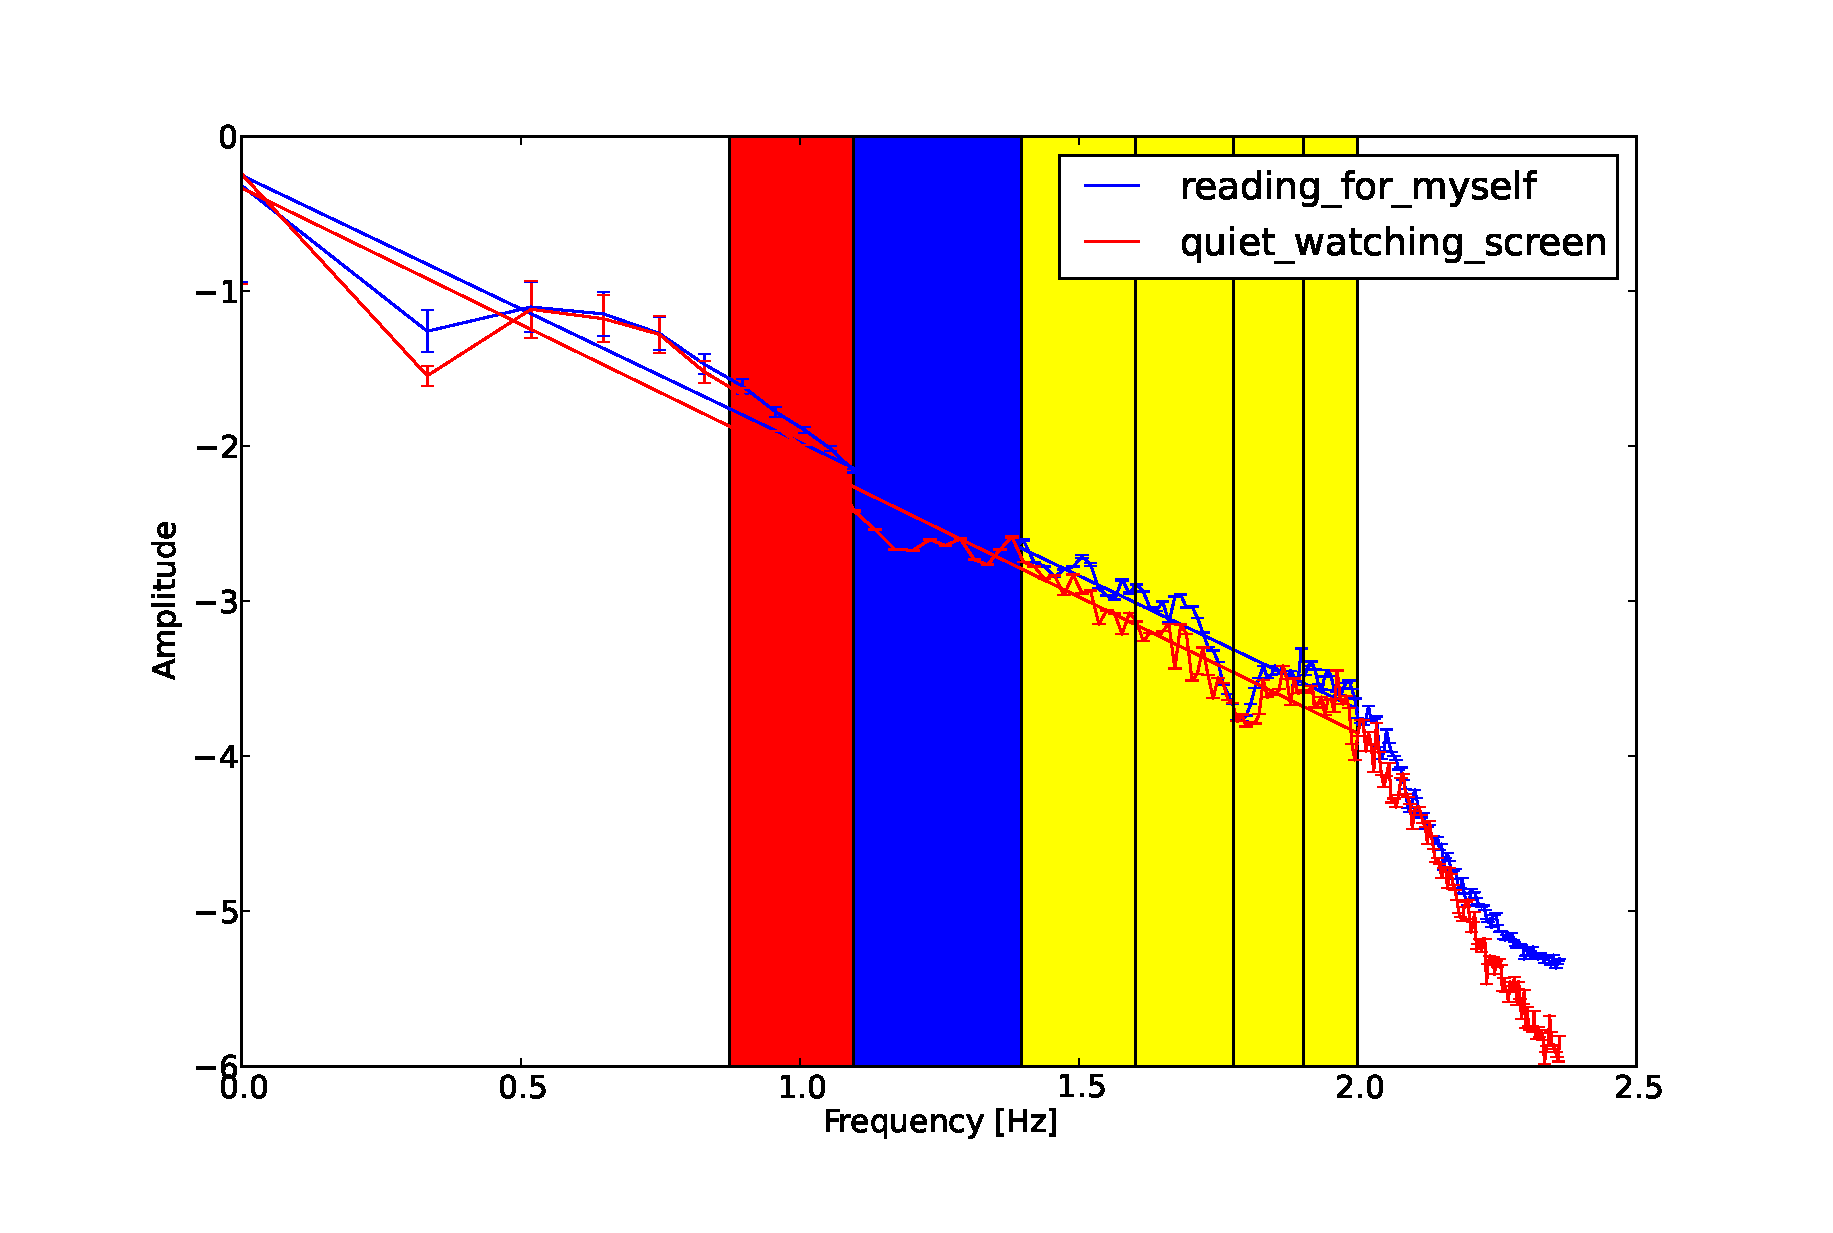
\includegraphics[width=0.9\columnwidth]{../figures/compare_pSpectra.eps}
\caption{Comparison of power spectra of a subject (i) resting state and (ii) reading a text in English for himself. {\bf [report the entropy values in both cases]}}
\label{fig:pspectrum}
\end{figure}


Then, entropy.

\begin{equation}
\label{eq:tsallis}
S_q(X) = \frac{1}{q-1} \left( 1 - \sum_{i=1}^n (p_i)^q \right).
\end{equation}

\begin{equation}
\label{eq:shannon}
S_1(X) = - \sum_{i=1}^n p_i\cdot log_{2}(p_i), ~~for~~q=1.
\end{equation}

\subsubsection{Why Entropy ?}

higher frequencies are usually associated to higher cognitive brain activation. Higher activation  translated into larger entropy $S$.


We wanted a lightweight mobile apparatus, which does not require complicated machine learning or any communication with a cloud service, or would not drain a battery. We purposely decided for a cheap update method {\bf [continue this point in discussion because it helps introduce future work]}

\begin{figure}[!t]
\centering
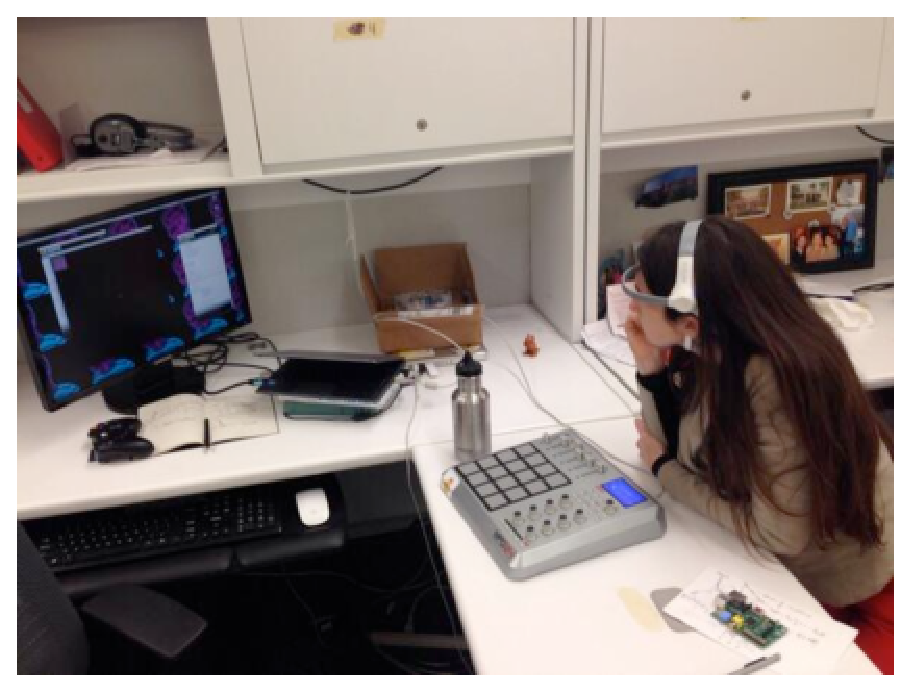
\includegraphics[width=0.9\columnwidth]{../figures/ariel.eps}
\caption{Ariel Garten (Interaxon / Muse CEO) playing with the brain speed reader.}
\label{fig:ariel}
\end{figure}

One could argue that we could have taken the {\it meditation} and {\it attention} metrics provided by Neurosky (and computed directly in the headset). However, these metrics are proprietary and their formula kept secret (we suspect nevertheless that they take $\alpha$ and $\beta$ waves  as an input). Furthermore, extensive testing did not allow us find any consistency with what we would quality meditation or attention. As a result, we preferred to stick to the principles of reproducible science.

\subsection{Negative Feedback Loop}

Explain: higher cog. activity  $\rightarrow$  higher entropy $\rightarrow$  lower word display rate $\rightarrow$ lower cog. activity. {\bf [probably not worth a section]}


\subsection{Word Display Rate Update}

\begin{equation}
\label{eq:Snormalized}
S_{norm}(t) = \frac{S(t) - \langle S \rangle}{\sigma_{S}}, 
\end{equation}
with $\langle S \rangle$ and $\sigma_{S}$ the average and standard deviation of the entropy $S$ calculated over the last 20 points (i.e., the last 5 seconds?). The normalization ensures that $S_{norm}$ is always centered around $0$. The rate $R(t+1)$ of word display is then updated as follows,

\begin{equation}
R(t+\Delta t) = R(t) \left[1 - \alpha \cdot S_{norm}(t)\right],
\label{eq:RateChange}
\end{equation}

where $\Delta t = 0.25$ seconds and $\alpha = 0.20$. In other words, the normalized entropy influences for 20\% the rate change $\Delta R =  \left[ R(t+\Delta t) - R(t) \right] / R(t) = - \alpha \cdot S_{norm}(t)$. Increasing $\alpha$ increases the influence of $S_{norm}$, and the negative sign ensures control of $R$ with a mean reverting process. Note however, that since $S_{norm}$ is calculated from a moving average on a rather short time window, $R$ exhibits excursions (c.f. Figure \ref{fig:trajectory}).

\begin{figure}[!t]
\centering
%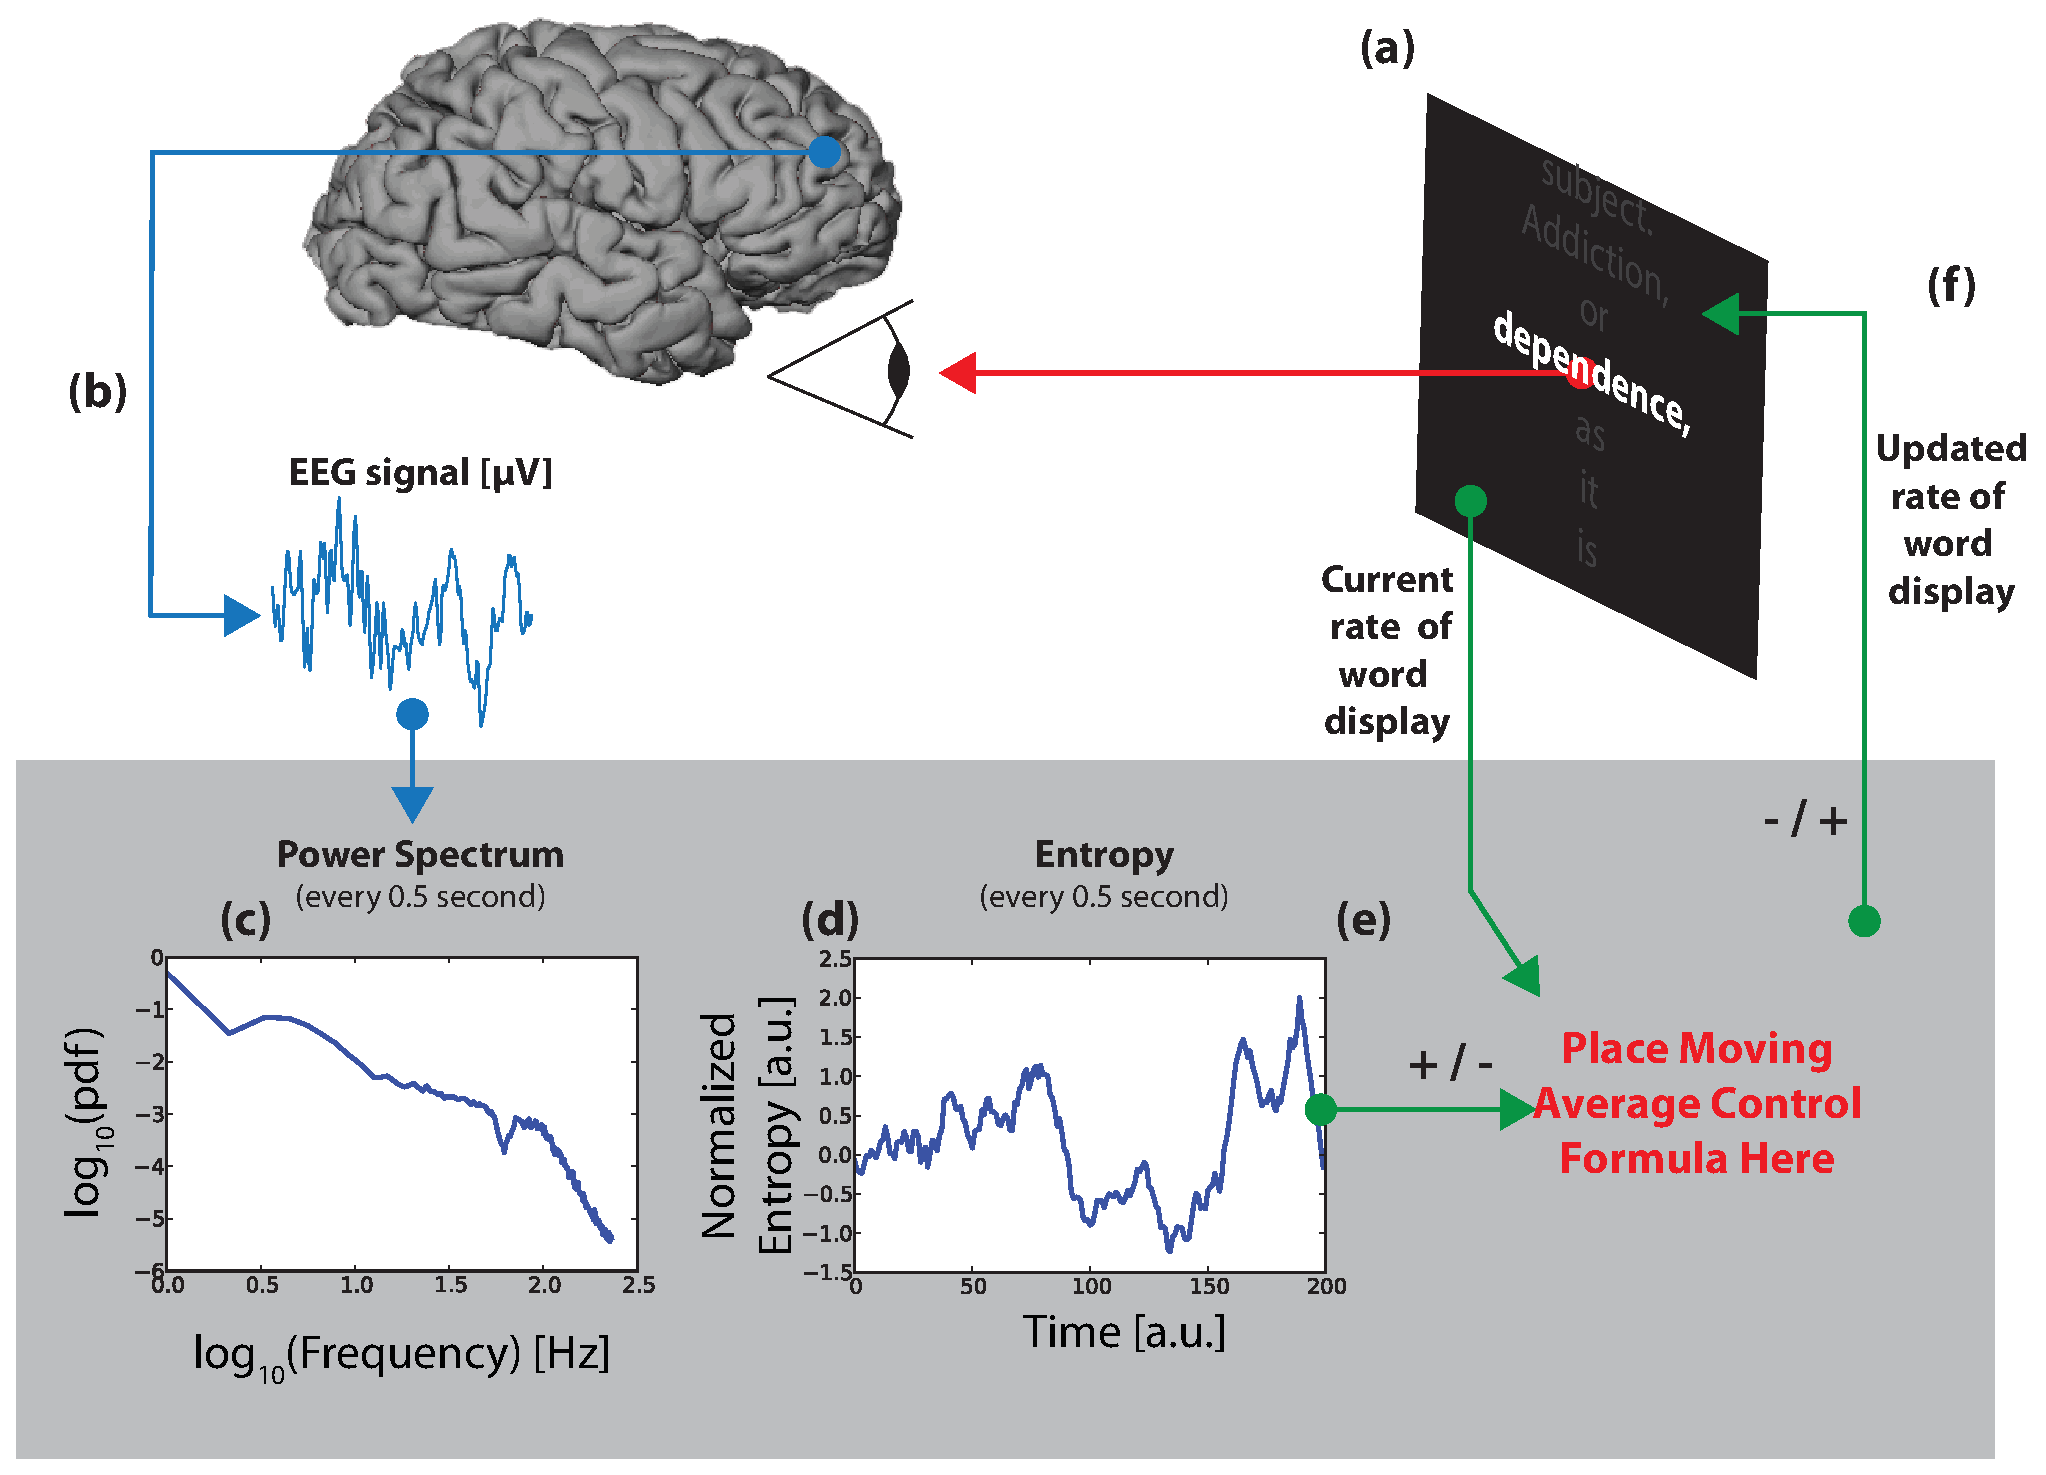
\includegraphics[width=0.9\columnwidth]{../figures/apparatus.eps}
\caption{typical evolution of rate $R$.}
\label{fig:trajectory}
\end{figure}

\section{Experimental Protocol}
To determine the gains of our brain speed-reader apparatus when reading, we have conducted an experiment, involving XX subjects who participated in our study. The experimental procedures described here were approved by an Institutional Review Board. 

\subsection{Procedure}
After obtaining individual consent, we conducted a quick {\bf calibration} task. A text was displayed word by word to each subject, who could adapt the rate of word display with the right (faster) and left (slower) arrow keys, until they reach their comfort zone. This baseline rate would be reused during the experiment. Then, the subject was asked to {\bf wear} the Neurosky Mindset. When ready, a {\bf text was displayed word by word} in a Rapid Visual Serial Presentation (RVSP) manner. After all text was been displayed, the subject was asked some comprehension questions regarding the content of the text. This procedure was repeated three or four times with various texts and various treatments involving varying the rate $R$ of word display:

\begin{enumerate}
  \item {\bf Constant Rate: } the rate of word display remains constant with $R(t) = R_{0}$ for $\forall t$.  
  \item {\bf Brainwave Treatment: } starting from the baseline $R_0$, the rate $R$ changes every quarter second as a function of the rate at the previous step and as a function of the entropy $S_{norm}$ measured in real-time from the EEG captured by the Neurosky mindset, and according to formula (\ref{eq:RateChange}).
    \item {\bf Random Rate Treatment: }  %Randomly Varying Text : R(1) $\rigtharrow$ AR1(n,baseline,baseline/2,0.5,sigma=std) AR1 formula : c + phi * X[-1] + np.random.normal(scale=sigma)
\end{enumerate}

The subject was wearing the Neurosky headset and was not informed whether the treatment involved using EEG as an input for controlling the rate $R$ of word display. In other word, the subject and no information on the three treatments, and had no possibility to distinguish between these treatments, in other ways than guessing from their experience.

In case, four treatments were applied, one of the treatments was repeated once with a different text. After the end, subjects were asked to fill short surveys for each text, asking about comfort, perceived level of understanding, degree of control, followed by a survey to collect demographic informations.

\subsection{Measuring Text Complexity}

ATOS  ( ref: Michael Milone,The Development of ATOS, The Renaissance Readability Formula, p10 (2010) \url{http://doc.renlearn.com/KMNet/R004250827GJ11C4.pdf}

\begin{itemize}
  \item Words per sentence
  \item Average grade level of words ( which class grade the word is first seen)
  \item Characters per word
\end{itemize}


$ATOS Rasch Difficulty Formula = -8.54 + 1.95 * Ln(AvgWords) + .46 * AvgGrad100 + 1.74 * Ln(AvgChar)$

Adjustment for books with less than 500 words

$BLGL for Books With Fewer Than 500 Words = .004 * Book Length + 0.4$


Table detailing texts : \url{https://docs.google.com/spreadsheets/d/1uwkoToM-p3UFrd0U_1vOX4eBJsmYuPVYVhvhsZ8Y5Nc/edit#gid=0}




%\begin{itemize}
%  \item {\bf text 0 (adapted from Coming of Age in Samoa, Margaret Mead, 1928
%)}:   $ATOS=9.5$,  $word~count = 421$
%  \item {\bf Text 1  (adapted from The Warden, Anthony Trollope, 1855)} : $ATOS=8.3$, $word~count = 563$
%  \item {\bf Text 2  (adapted from The Mayor of Casterbridge, Thomas Hardy, 1886) } : $ATOS=10.2$, $word~count = 831$
%  \item {\bf Text 3 (Adapted from: The Social Function of Science, John D Bernal (1939))} : $ATOS=11.9$, $word~count = 421$
%\end{itemize}



\begin{figure}[!t]
\centering
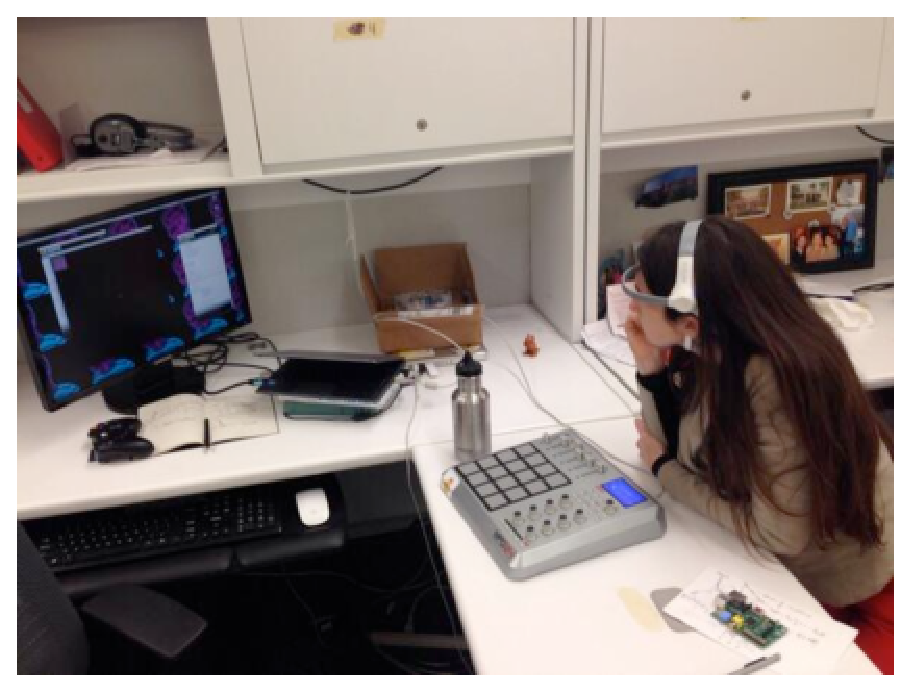
\includegraphics[width=0.9\columnwidth]{../figures/ariel.eps}
\caption{Show a picture with someone taking the experiment.}
\label{fig:ariel}
\end{figure}



